\chapter{Arquitetura do Projeto}
\label{arq-cap}
Este capítulo descreve o funcionamento de cada componente do GSMART. A
\autoref{esquema-geral} representa um esquema geral dos módulos do projeto, já a
\autoref{diagrama-fluxo} apresenta o mesmo esquema da visão de um diagrama de
fluxo, sendo apontados entidades e processos do sistema.

\begin{figure}[!h]
  \caption{\label{esquema-geral}Arquitetura geral do sistema}
  \begin{center}
    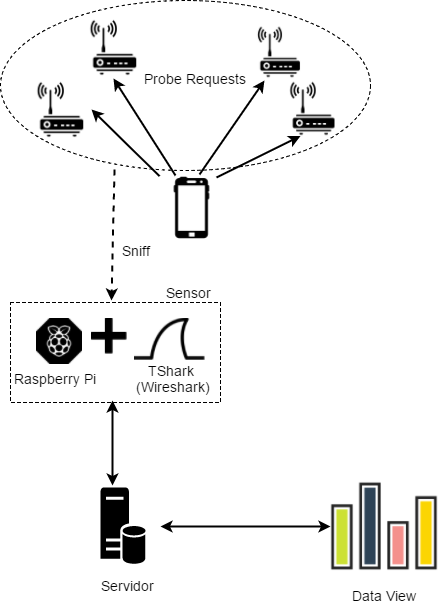
\includegraphics[width=0.50\textwidth]{img/esquema_geral.png}
  \end{center}
  \legend{Fonte: Elaborada pelas autoras.}
\end{figure}

\begin{figure}[!h]
  \caption{\label{diagrama-fluxo}Diagrama de Fluxo}
  \begin{center}
    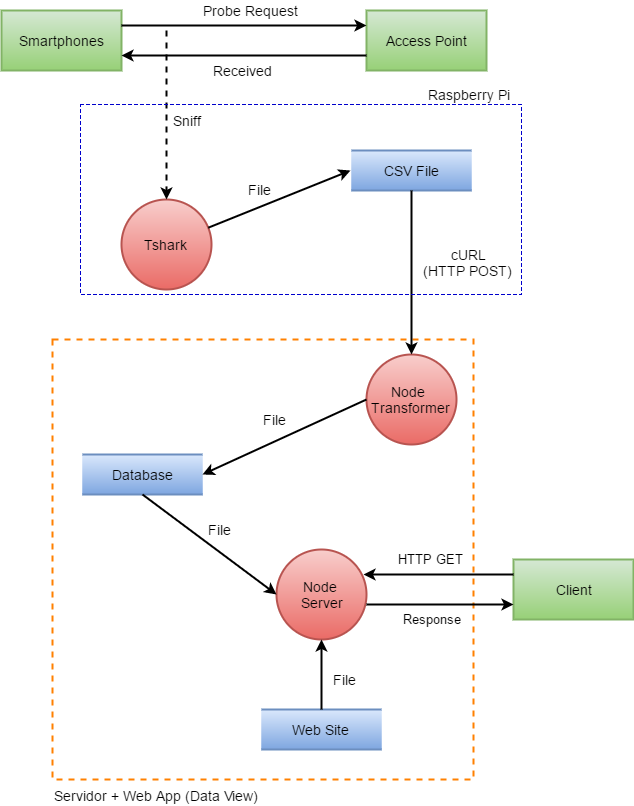
\includegraphics[width=0.70\textwidth]{img/diagrama_fluxo.png}
  \end{center}
  \legend{Fonte: Elaborada pelas autoras.}
\end{figure}


\section{Sensor}
\label{secao-sensor}
O módulo Sensor é um processo que roda num Raspberry Pi Model 3 B equipado de
uma antena Ralink no modo monitor. Este processo é um programa escrito em
Node.js que: habilita o modo monitor da antena, executa comandos Tshark para capturar de pacotes
\emph{probe request}, salva os endereços MAC
capturados num arquivo que, posteriormente, é recuperado do diretório de
arquivos (\emph{Files Directory}) e enviado ao servidor.

\begin{figure}[!h]
  \caption{\label{trecho-sensor}Trecho de código do sensor}
  \begin{center}
    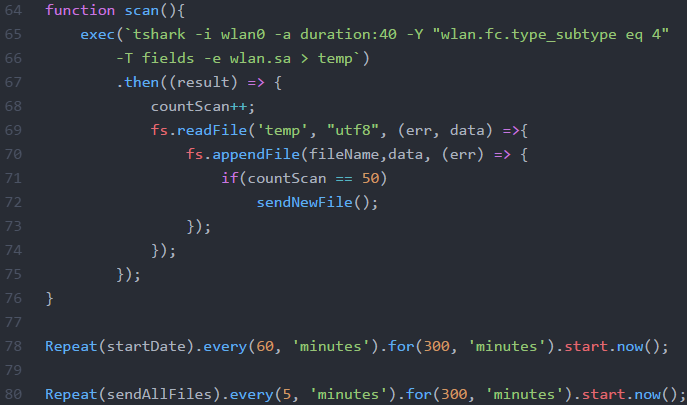
\includegraphics[width=1.0\textwidth]{img/sensor.png}
  \end{center}
  \legend{Fonte: Elaborada pelas autoras.}
\end{figure}

A \autoref{trecho-sensor} contém uma parte do código que executa dentro do
sensor. Ele funciona em 3 fluxos:

\begin{itemize}
    \item \textbf{startDate}: esse fluxo, representado na linha 78
    do código, executa a função "startDate" cada 60 minutos, criando um arquivo com
    o nome "ZONA\_YYYY-MM-DD\_HH:00", especificando zona, dia e hora de detecção. Logo
    após, salva o arquivo e inicia o fluxo a seguir;
    \item \textbf{scan}: este fluxo (linha 78) repete a função "scan" a cada 40 segundos durante 50 minutos que executa o
    comando Tshark (veja \autoref{tshark-section}) que vai armazenando os endereço
    MAC num arquivo temporário. Quando as execuções do Tshark chegam na contagem 50
    o conteúdo do arquivo  é copiado para o arquivo gerado no fluxo anterior, então é enviado ao servidor;
    \item \textbf{sendAllFiles}: este fluxo (linha 80) repete a função "sendAllFiles" a cada 5 minutos enviando todos os arquivos que tiveram falha no seu
    primeiro envio.
    capturado.
\end{itemize}

\section{Node Transformer}
\label{node-transformer}
Após receber o arquivo, o servidor salva-o no diretório e encaminha os endereços MAC capturados para o
módulo de transformação.

O Node Transformer é um módulo dentro do \emph{webserver}
que transforma os endereços MAC em dados formatados.
de dados. Primeiro, são eliminadas os endereços repetidos. Depois, a estrutura de dado (objeto)
que representa um registro do banco é preenchida com a informações. Uma parte importante dessa preparação
é que o fabricante de cada dispositivo é obtido através de uma API\footnote{\url{https://macvendors.com/}} de consulta de endereços MAC. Por fim,
o objeto preenchido é salvo no banco de dados.

\subsection{Formatação do dado}
A formatação do dado foi pensada de acordo com a unidade de tratamento escolhida para a medição tráfego, o dia.
Dentro da aplicação e do banco, o dado possui o formato do JSON da \autoref{formatacao-dado}.

\begin{figure}[!h]
  \caption{\label{formatacao-dado}Formatação do dado}
  \begin{center}
    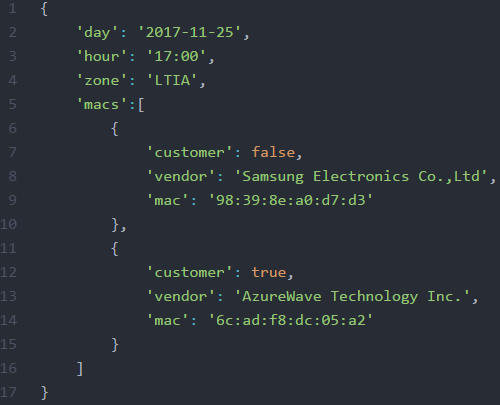
\includegraphics[width=0.8\textwidth]{img/formato-dado.png}
  \end{center}
  \legend{Fonte: Elaborada pelas autoras.}
\end{figure}

Cada objeto como o da \autoref{formatacao-dado}, possui os seguintes campos sobre a medição:
\begin{itemize}
    \item \textbf{day}: dia;
    \item \textbf{hour}: hora;
    \item \textbf{zone}: zona em que foi realizada;
    \item \textbf{macs}: vetor de todos os endereços MAC capturados;
    \item \textbf{customer}: se o endereço captado já foi capturado outro(s) dia(s);
    \item \textbf{vendor}: fabricante do dispositivo;
    \item \textbf{mac}: endereços MAC.
\end{itemize}

O maior ganho com essa formatação é durante as \emph{queries} e processamento dos dados. O dado pode ser recuperado
por zona ou por dia, dependendo da visualização de dados selecionada.

\section{Node Server}
\label{node-server}
Este módulo que engloba o módulo da \autoref{node-transformer}, também: define
quais recursos recursos da aplicação são acessadas pelo cliente e como os dados
são processados segundo cada visualização de dados.

\subsection{Deliberando recursos}
O Node Server é um \emph{web service} baseado no padrão REST (Representational
State Transfer, em português Transferência de Estado Representacional). Adotando
esse padrão implica que temos uma RESTful API \cite{pires2017}. De modo geral, a aplicação define
URIs que através de verbos HTTP (GET e POST), fornecem à requisão do cliente
algum recurso específico. Por exemplo, ao acessar a URL do servidor acompanhado de "/statistics/LTIA", a API
desenvolvida responde ao cliente com uma página HTML com informações referentes a zona LTIA.

Todas as URIs possíveis foram definidas através de um \emph{middleware} com o
pacote do Node, o Express.js\footnote{\url{http://expressjs.com/}}. Este emprega rotas para definir quais recursos
serão fornecidos ao cliente. Na \autoref{trecho-express} temos o exemplo de trecho de código do \emph{middleware} da
aplicação. Nesse exemplo, assim que o servidor recebe um requisição HTTP GET, após um processamento de dados, responde
ao cliente com a visualização de dados ``statistics'' com o dado em forma de JSON (linha 5). Já \autoref{rotas} descreve
todas as rotas (URIs) acessíveis ao cliente.

\begin{figure}[!h]
  \caption{\label{trecho-express}\emph{Middleware} com Express.js}
  \begin{center}
    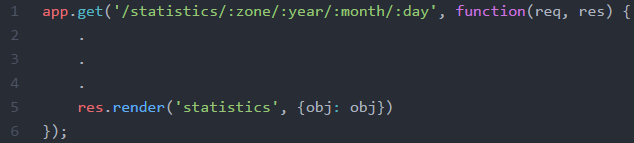
\includegraphics[width=1.0\textwidth]{img/trecho-express.png}
  \end{center}
  \legend{Fonte: Elaborada pelas autoras.}
\end{figure}

\begin{figure}[!h]
  \caption{\label{rotas}Rotas do Express}
  \begin{center}
    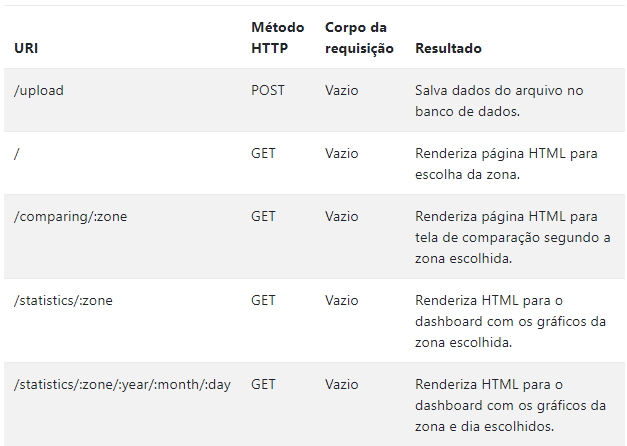
\includegraphics[width=1.0\textwidth]{img/rotas.png}
  \end{center}
  \legend{Fonte: Elaborada pelas autoras.}
\end{figure}

\subsection{Processando dados}
Além de deliberar recursos, o Node Serve recupera os dados e processá-os para
apresentar ao usuário. Assim que o cliente faz a requisição ao servidor, dados
referentes à zona e/ou dia selecionados são recuperados do banco de dados. Em
seguida, esses elementos passam por outros módulos que retornam JSON com as
informações necessárias para apresentar ao usuários.

\section{Visualização de Dados}
\label{data-view}
Assim que o cliente faz requisição ao servidor, dependendo da rota que ele tentou acessar será direcionado
a diferentes visualizações de dados.

Cada visualização de dados é uma página HTML construída pela
linguagem de \emph{template} EJS\footnote{\url{http://www.embeddedjs.com/}} (Embedded JavaScript) cuja função é
auxiliar na injeção de conteúdo (dado) na página requisitada.

Quando o cliente acessa uma rota, o servidor recebe a requisição, passa para os
módulos de processamento de dados e, então renderiza a \emph{view} (visualização de dados) correta. Cada
uma das visualizações serão apresentadas a seguir.

\subsection{Seleção de zona}
\label{seleciona-zona}
Nessa tela, o usuário seleciona a zona da qual deseja informação. As zonas disponíveis para aplicação são:
"HOMEJ", "HOMEC", "LTIA" e "Camflam".

\begin{figure}[!h]
  \caption{\label{zones-ap}Tela de seleção de zonas}
  \begin{center}
    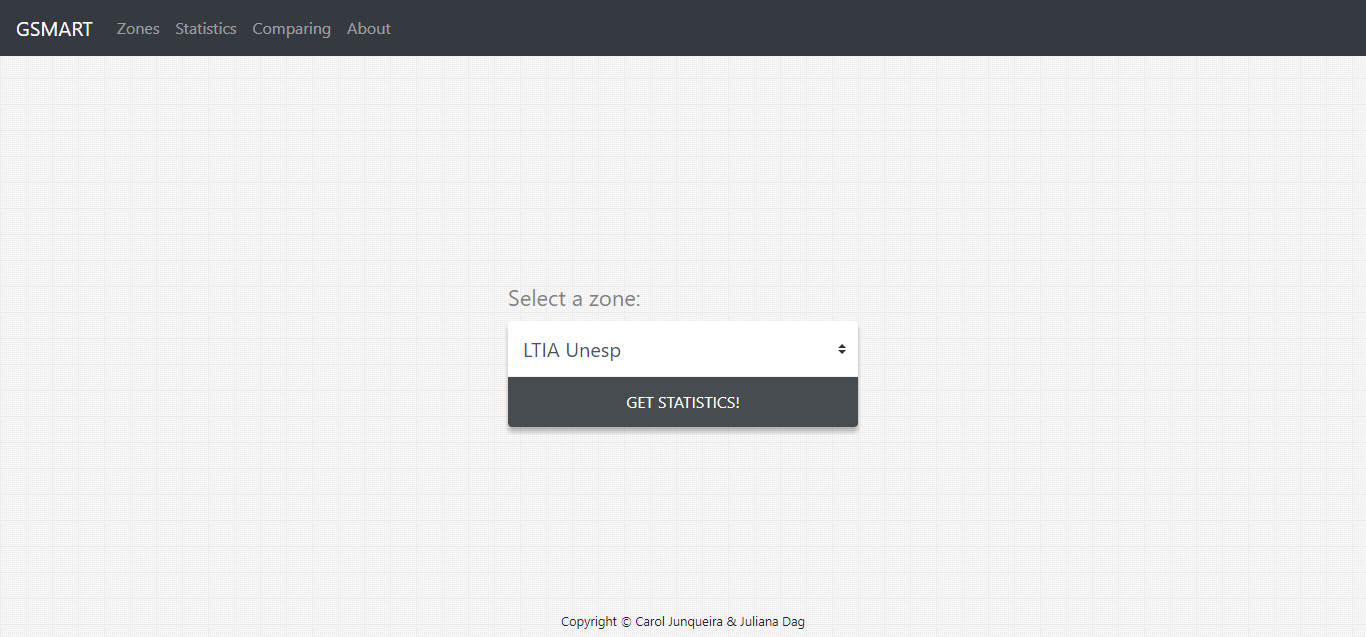
\includegraphics[width=1.0\textwidth]{img/zones.png}
  \end{center}
  \legend{Fonte: Elaborada pelas autoras.}
\end{figure}

\subsection{Estatística diária}
\label{diaria}
Após ter selecionado uma zona na tela da \autoref{seleciona-zona}, o usuário é
redirecionado para a página exposta na \autoref{statistics-ap}. Nesta
\emph{view} são apresentadas informações referentes a cada dia de captura
realizado para aquela área.

No canto superior esquerdo da \autoref{statistics-ap}, é possível ver a zona
escolhida, além disso, pode-se selecionar o dia para visualizar as estatísticas
no espaço reservado. O gráfico de curva representa crescimento do tráfego de pessoas ao longo das
horas registradas. Já o gráfico setores apresenta o número e porcentagem de dispositivos por fabricante.

\begin{figure}[!h]
  \caption{\label{statistics-ap}\emph{Dashboard}}
  \begin{center}
    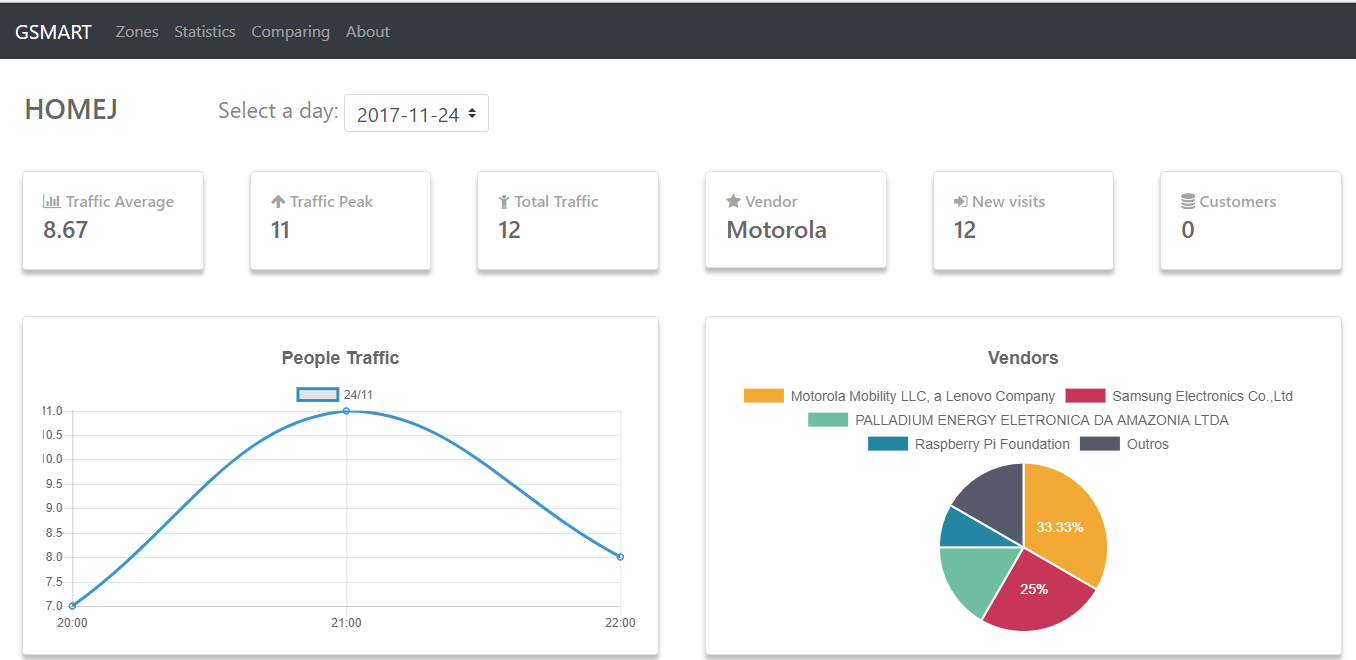
\includegraphics[width=1.0\textwidth]{img/statistics.png}
  \end{center}
  \legend{Fonte: Elaborada pelas autoras.}
\end{figure}

Neste trabalho foram selecionadas algumas informações com base nos estudos de \emph{geomarketing} que seriam
de expressividade e relevância para o usuário. Essas informações são, de acordo com a ordem disposta
na figura:

\begin{itemize}
    \item \textbf{Traffic Average}: é a média de tráfego de pessoas por hora;
    \item \textbf{Traffic Peak}: é o maior valor de detecção dentro do intervalo de horas disponíveis;
    \item \textbf{Total Traffic}: é o número total de indivíduos (diferentes) dentre todas as horas escaneadas;
    \item \textbf{Vendor}: fabricante de dispositivo móvel detectado em maior número;
    \item \textbf{New Visits}: do total de indivíduos quantos estão presentes pela primeira vez;
    \item \textbf{Customers}: número total de pessoas que já estiveram alguma vez dentro daquela zona, considera
    só os dias anteriores.
\end{itemize}

\subsection{Comparação de dias}
Para facilitar a comparação de todos os dias de captura de uma zona, há uma tela de comparação, como mostra
a \autoref{comparing-ap}. Esta tela mostra num gráfico de barras todos os dias e seus respectivos número
de dispositivos por hora. Numa mesma hora é possível ter a plotagem de várias barras para verificar
a diferenças e semelhanças entre os dias. Logo abaixo, há uma tabela que apresenta todas as informações
contidas na \emph{view} de estatísticas diárias (veja \autoref{diaria}) para todos os dias disponíveis dentro
da zona.

No canto superior esquerdo da tela há um espaço reservado para a mudança de zona.

\begin{figure}[!h]
  \caption{\label{comparing-ap}Tela de Comparação}
  \begin{center}
    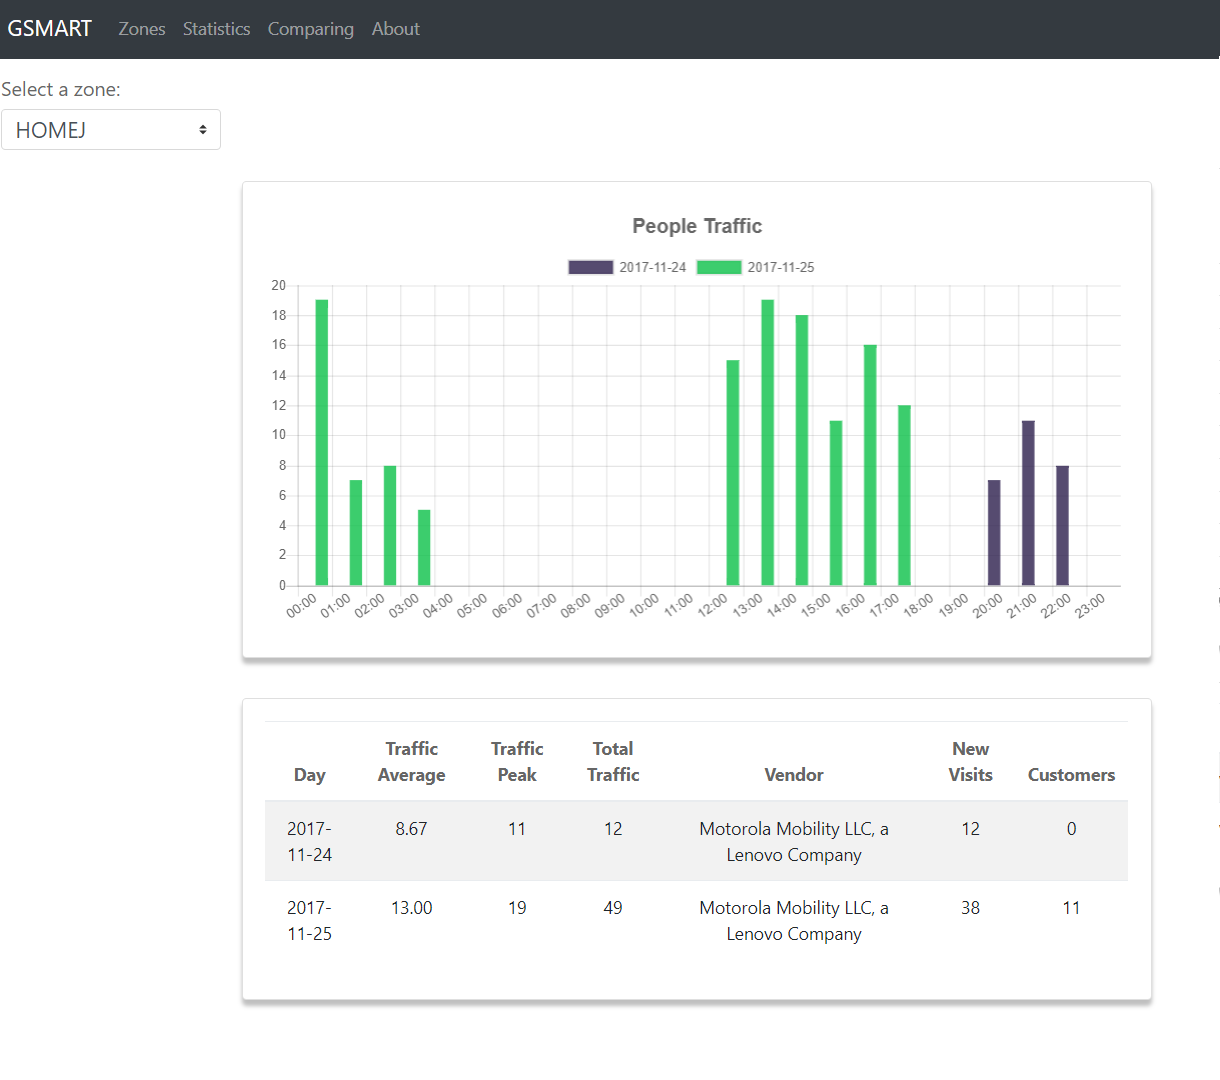
\includegraphics[width=1.0\textwidth]{img/comparing.png}
  \end{center}
  \legend{Fonte: Elaborada pelas autoras.}
\end{figure}

\section{Arquitura MVC}
Para estruturar todos os módulos do projeto foi utilizada a arquitetura de
software MVC (Model View Controller) que é amplamente usado com os utilizados
Express.js e Node.js, tendo exemplos da comunidade e dentro da documentação dessas
tecnologias.

O MVC divide a aplicação em três componentes- Model, View e Controller -
promovendo modularidade e facilidade de colaoração e reutilização \cite{mdn}. Cada componente represeta:

\begin{itemize}
    \item \textbf{Model}: armazena os dados da aplicação e notifica as \emph{views} e
    \emph{controllers} sobre a mudança de estados desses dados. Sendo assim, as visualizações e os controladores
    podem tomar ações, como, atualizar a visão dos dados e executar comandos, respectivamente.
    \item \textbf{Views}: apresentam aos usuários as informações e é um meio de interação deles com
    a aplicação;
    \item \textbf{Controllers}: atualizam os \emph{models} e \emph{views} de acordo
    com atualizações de dados pela própria aplicação ou por interação com o usuário.
\end{itemize}

No caso deste projeto, os \emph{models} foram construídos através do pacote do Node.js que auxilia
na manipulação de dados do MongoDB, o Mongoose\footnote{\url{http://mongoosejs.com/}}. Já todas as \emph{views}
foram construídas com a linguagem de template EJS e HTML. A linguagem Javascript foi utiliza para o desenvolvimento
de todos esses componentes, facilitando pelo uso tanto do lado do servidor como a do cliente.
